% Options for packages loaded elsewhere
% Options for packages loaded elsewhere
\PassOptionsToPackage{unicode}{hyperref}
\PassOptionsToPackage{hyphens}{url}
%
\documentclass[
  english,
  russian,
  12pt,
  a4paper,
  DIV=11,
  numbers=noendperiod]{scrreprt}
\usepackage{xcolor}
\usepackage[margin=2cm]{geometry}
\usepackage{amsmath,amssymb}
\setcounter{secnumdepth}{5}
\usepackage{iftex}
\ifPDFTeX
  \usepackage[T1]{fontenc}
  \usepackage[utf8]{inputenc}
  \usepackage{textcomp} % provide euro and other symbols
\else % if luatex or xetex
  \usepackage{unicode-math} % this also loads fontspec
  \defaultfontfeatures{Scale=MatchLowercase}
  \defaultfontfeatures[\rmfamily]{Ligatures=TeX,Scale=1}
\fi
\usepackage{lmodern}
\ifPDFTeX\else
  % xetex/luatex font selection
  \setmainfont[]{DejaVu Sans}
  \setmonofont[]{DejaVu Sans Mono}
\fi
% Use upquote if available, for straight quotes in verbatim environments
\IfFileExists{upquote.sty}{\usepackage{upquote}}{}
\IfFileExists{microtype.sty}{% use microtype if available
  \usepackage[]{microtype}
  \UseMicrotypeSet[protrusion]{basicmath} % disable protrusion for tt fonts
}{}
\usepackage{setspace}
% Make \paragraph and \subparagraph free-standing
\makeatletter
\ifx\paragraph\undefined\else
  \let\oldparagraph\paragraph
  \renewcommand{\paragraph}{
    \@ifstar
      \xxxParagraphStar
      \xxxParagraphNoStar
  }
  \newcommand{\xxxParagraphStar}[1]{\oldparagraph*{#1}\mbox{}}
  \newcommand{\xxxParagraphNoStar}[1]{\oldparagraph{#1}\mbox{}}
\fi
\ifx\subparagraph\undefined\else
  \let\oldsubparagraph\subparagraph
  \renewcommand{\subparagraph}{
    \@ifstar
      \xxxSubParagraphStar
      \xxxSubParagraphNoStar
  }
  \newcommand{\xxxSubParagraphStar}[1]{\oldsubparagraph*{#1}\mbox{}}
  \newcommand{\xxxSubParagraphNoStar}[1]{\oldsubparagraph{#1}\mbox{}}
\fi
\makeatother

\usepackage{color}
\usepackage{fancyvrb}
\newcommand{\VerbBar}{|}
\newcommand{\VERB}{\Verb[commandchars=\\\{\}]}
\DefineVerbatimEnvironment{Highlighting}{Verbatim}{commandchars=\\\{\}}
% Add ',fontsize=\small' for more characters per line
\usepackage{framed}
\definecolor{shadecolor}{RGB}{241,243,245}
\newenvironment{Shaded}{\begin{snugshade}}{\end{snugshade}}
\newcommand{\AlertTok}[1]{\textcolor[rgb]{0.68,0.00,0.00}{#1}}
\newcommand{\AnnotationTok}[1]{\textcolor[rgb]{0.37,0.37,0.37}{#1}}
\newcommand{\AttributeTok}[1]{\textcolor[rgb]{0.40,0.45,0.13}{#1}}
\newcommand{\BaseNTok}[1]{\textcolor[rgb]{0.68,0.00,0.00}{#1}}
\newcommand{\BuiltInTok}[1]{\textcolor[rgb]{0.00,0.23,0.31}{#1}}
\newcommand{\CharTok}[1]{\textcolor[rgb]{0.13,0.47,0.30}{#1}}
\newcommand{\CommentTok}[1]{\textcolor[rgb]{0.37,0.37,0.37}{#1}}
\newcommand{\CommentVarTok}[1]{\textcolor[rgb]{0.37,0.37,0.37}{\textit{#1}}}
\newcommand{\ConstantTok}[1]{\textcolor[rgb]{0.56,0.35,0.01}{#1}}
\newcommand{\ControlFlowTok}[1]{\textcolor[rgb]{0.00,0.23,0.31}{\textbf{#1}}}
\newcommand{\DataTypeTok}[1]{\textcolor[rgb]{0.68,0.00,0.00}{#1}}
\newcommand{\DecValTok}[1]{\textcolor[rgb]{0.68,0.00,0.00}{#1}}
\newcommand{\DocumentationTok}[1]{\textcolor[rgb]{0.37,0.37,0.37}{\textit{#1}}}
\newcommand{\ErrorTok}[1]{\textcolor[rgb]{0.68,0.00,0.00}{#1}}
\newcommand{\ExtensionTok}[1]{\textcolor[rgb]{0.00,0.23,0.31}{#1}}
\newcommand{\FloatTok}[1]{\textcolor[rgb]{0.68,0.00,0.00}{#1}}
\newcommand{\FunctionTok}[1]{\textcolor[rgb]{0.28,0.35,0.67}{#1}}
\newcommand{\ImportTok}[1]{\textcolor[rgb]{0.00,0.46,0.62}{#1}}
\newcommand{\InformationTok}[1]{\textcolor[rgb]{0.37,0.37,0.37}{#1}}
\newcommand{\KeywordTok}[1]{\textcolor[rgb]{0.00,0.23,0.31}{\textbf{#1}}}
\newcommand{\NormalTok}[1]{\textcolor[rgb]{0.00,0.23,0.31}{#1}}
\newcommand{\OperatorTok}[1]{\textcolor[rgb]{0.37,0.37,0.37}{#1}}
\newcommand{\OtherTok}[1]{\textcolor[rgb]{0.00,0.23,0.31}{#1}}
\newcommand{\PreprocessorTok}[1]{\textcolor[rgb]{0.68,0.00,0.00}{#1}}
\newcommand{\RegionMarkerTok}[1]{\textcolor[rgb]{0.00,0.23,0.31}{#1}}
\newcommand{\SpecialCharTok}[1]{\textcolor[rgb]{0.37,0.37,0.37}{#1}}
\newcommand{\SpecialStringTok}[1]{\textcolor[rgb]{0.13,0.47,0.30}{#1}}
\newcommand{\StringTok}[1]{\textcolor[rgb]{0.13,0.47,0.30}{#1}}
\newcommand{\VariableTok}[1]{\textcolor[rgb]{0.07,0.07,0.07}{#1}}
\newcommand{\VerbatimStringTok}[1]{\textcolor[rgb]{0.13,0.47,0.30}{#1}}
\newcommand{\WarningTok}[1]{\textcolor[rgb]{0.37,0.37,0.37}{\textit{#1}}}

\usepackage{longtable,booktabs,array}
\newcounter{none} % for unnumbered tables
\usepackage{calc} % for calculating minipage widths
% Correct order of tables after \paragraph or \subparagraph
\usepackage{etoolbox}
\makeatletter
\patchcmd\longtable{\par}{\if@noskipsec\mbox{}\fi\par}{}{}
\makeatother
% Allow footnotes in longtable head/foot
\IfFileExists{footnotehyper.sty}{\usepackage{footnotehyper}}{\usepackage{footnote}}
\makesavenoteenv{longtable}
\usepackage{graphicx}
\makeatletter
\newsavebox\pandoc@box
\newcommand*\pandocbounded[1]{% scales image to fit in text height/width
  \sbox\pandoc@box{#1}%
  \Gscale@div\@tempa{\textheight}{\dimexpr\ht\pandoc@box+\dp\pandoc@box\relax}%
  \Gscale@div\@tempb{\linewidth}{\wd\pandoc@box}%
  \ifdim\@tempb\p@<\@tempa\p@\let\@tempa\@tempb\fi% select the smaller of both
  \ifdim\@tempa\p@<\p@\scalebox{\@tempa}{\usebox\pandoc@box}%
  \else\usebox{\pandoc@box}%
  \fi%
}
% Set default figure placement to htbp
\def\fps@figure{htbp}
\makeatother



\ifLuaTeX
\usepackage[bidi=basic,shorthands=off,provide=*]{babel}
\else
\usepackage[bidi=default,shorthands=off,provide=*]{babel}
\fi
\ifPDFTeX
\else
\babelfont{rm}[]{DejaVu Sans}
\fi
\ifLuaTeX
  \usepackage{selnolig} % disable illegal ligatures
\fi


\setlength{\emergencystretch}{3em} % prevent overfull lines

\providecommand{\tightlist}{%
  \setlength{\itemsep}{0pt}\setlength{\parskip}{0pt}}



 
\usepackage[style=gost-numeric,backend=biber,langhook=extras,autolang=other*]{biblatex}
\addbibresource{bib/cite.bib}

\usepackage[]{csquotes}

\usepackage{indentfirst}
\usepackage{float}
\floatplacement{figure}{H}
\IfFileExists{plex-otf.sty}{
  %% Full TeXlive
  \usepackage[
    % math,
    RM={Scale=0.94},SS={Scale=0.94},SScon={Scale=0.94},TT={Scale=MatchLowercase,FakeStretch=0.9},
    DefaultFeatures={Ligatures=Common}
  ]{plex-otf}
  % \usepackage[Scale=MatchUppercase]{juliamono}
}{
  %% TinyTeX
  \usepackage{libertine}
}
\KOMAoption{captions}{tableheading}
\makeatletter
\@ifpackageloaded{caption}{}{\usepackage{caption}}
\AtBeginDocument{%
\ifdefined\contentsname
  \renewcommand*\contentsname{Содержание}
\else
  \newcommand\contentsname{Содержание}
\fi
\ifdefined\listfigurename
  \renewcommand*\listfigurename{Список иллюстраций}
\else
  \newcommand\listfigurename{Список иллюстраций}
\fi
\ifdefined\listtablename
  \renewcommand*\listtablename{Список таблиц}
\else
  \newcommand\listtablename{Список таблиц}
\fi
\ifdefined\figurename
  \renewcommand*\figurename{Рисунок}
\else
  \newcommand\figurename{Рисунок}
\fi
\ifdefined\tablename
  \renewcommand*\tablename{Таблица}
\else
  \newcommand\tablename{Таблица}
\fi
}
\@ifpackageloaded{float}{}{\usepackage{float}}
\floatstyle{ruled}
\@ifundefined{c@chapter}{\newfloat{codelisting}{h}{lop}}{\newfloat{codelisting}{h}{lop}[chapter]}
\floatname{codelisting}{Список}
\newcommand*\listoflistings{\listof{codelisting}{Листинги}}
\makeatother
\makeatletter
\makeatother
\makeatletter
\@ifpackageloaded{caption}{}{\usepackage{caption}}
\@ifpackageloaded{subcaption}{}{\usepackage{subcaption}}
\makeatother
\usepackage{bookmark}
\IfFileExists{xurl.sty}{\usepackage{xurl}}{} % add URL line breaks if available
\urlstyle{same}
% fallback for those not using the hyperref driver hyperxmp:
\makeatletter
\@ifundefined{xmpquote}{\newcommand{\xmpquote}[1]{#1}}{}
\makeatother
\hypersetup{
  pdftitle={Лабораторная работа № 6},
  pdfauthor={Нечаева Кира Андреевна},
  pdflang={ru-RU},
  hidelinks,
  pdfcreator={LaTeX via pandoc}}


\title{Лабораторная работа № 6}
\usepackage{etoolbox}
\makeatletter
\providecommand{\subtitle}[1]{% add subtitle to \maketitle
  \apptocmd{\@title}{\par {\large #1 \par}}{}{}
}
\makeatother
\subtitle{Реализация модели SIR в подходе сетей Петри}
\author{Нечаева Кира Андреевна}
\date{2026-10-08}
\begin{document}
\maketitle

\renewcommand*\contentsname{Содержание}
{
\setcounter{tocdepth}{1}
\tableofcontents
}
\listoffigures
\listoftables

\setstretch{1.5}
\chapter{Цель
работы}\label{ux446ux435ux43bux44c-ux440ux430ux431ux43eux442ux44b}

Цель лабораторной работы --- реализовать эпидемиологическую модель SIR
средствами сетей Петри и исследовать её поведение при детерминированном
и стохастическом моделировании.

В модели используются три состояния: восприимчивые \texttt{S},
инфицированные \texttt{I} и выздоровевшие \texttt{R}. Переход
\texttt{infection} моделирует заражение, а переход \texttt{recovery} ---
выздоровление.

Дополнительно исследуется влияние коэффициента заражения, строится
анимация динамики модели и проводится расчёт для набора параметров.

\chapter{Подготовка рабочего
окружения}\label{ux43fux43eux434ux433ux43eux442ux43eux432ux43aux430-ux440ux430ux431ux43eux447ux435ux433ux43e-ux43eux43aux440ux443ux436ux435ux43dux438ux44f}

Работа выполнялась в Ubuntu через WSL. Проект расположен в общем
репозитории лабораторных работ и ведётся в ветке \texttt{develop}.

\begin{figure}[H]

{\centering 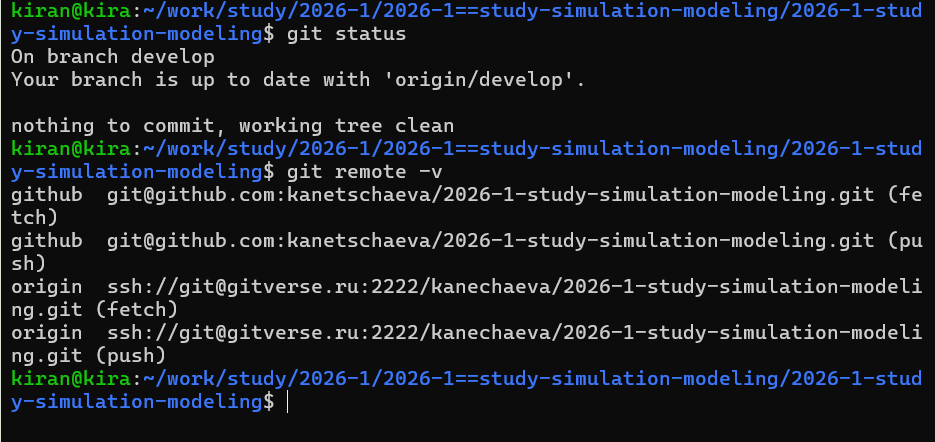
\includegraphics[width=0.95\linewidth,height=\textheight,keepaspectratio]{image/1.png}

}

\caption{Начальное состояние Git и удалённые репозитории}

\end{figure}%

Для работы были установлены библиотеки \texttt{AlgebraicPetri},
\texttt{Catlab}, \texttt{OrdinaryDiffEq}, \texttt{DataFrames},
\texttt{Plots}, \texttt{CSV}, а также средства литературного
программирования и Jupyter Notebook.

\begin{figure}[H]

{\centering 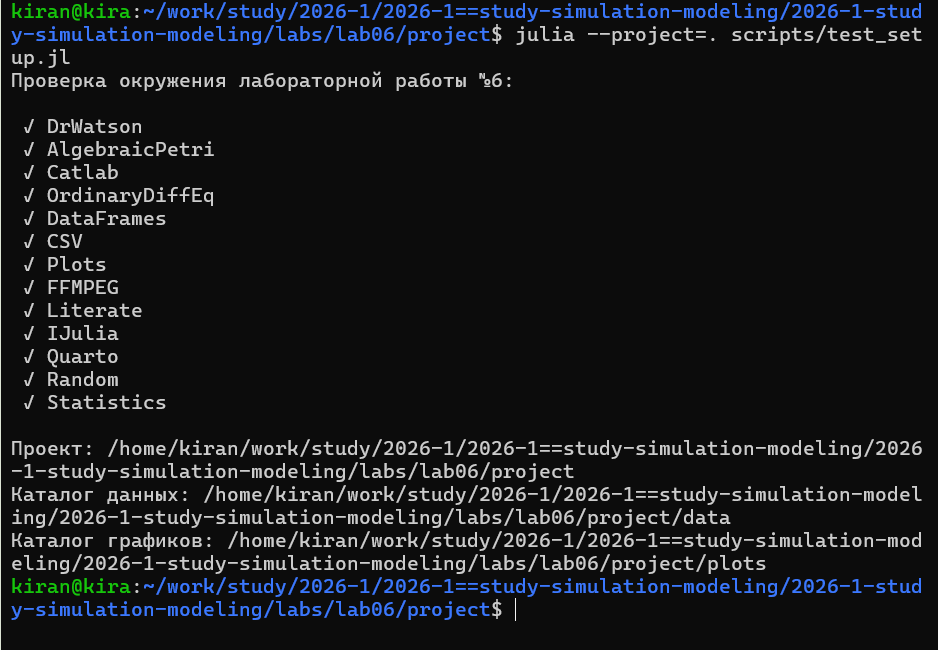
\includegraphics[width=0.95\linewidth,height=\textheight,keepaspectratio]{image/2.png}

}

\caption{Проверка рабочего окружения}

\end{figure}%

\chapter{Реализация сети Петри
SIR}\label{ux440ux435ux430ux43bux438ux437ux430ux446ux438ux44f-ux441ux435ux442ux438-ux43fux435ux442ux440ux438-sir}

Для модели определены три состояния:

\begin{itemize}
\tightlist
\item
  \texttt{S} --- восприимчивые;
\item
  \texttt{I} --- инфицированные;
\item
  \texttt{R} --- выздоровевшие.
\end{itemize}

Используются два перехода:

\begin{itemize}
\tightlist
\item
  \texttt{infection}: заражение восприимчивого при взаимодействии с
  инфицированным;
\item
  \texttt{recovery}: переход инфицированного в состояние выздоровления.
\end{itemize}

Начальная маркировка задаётся как:

\texttt{S\ =\ 990}, \texttt{I\ =\ 10}, \texttt{R\ =\ 0}.

Перед основными экспериментами была выполнена отдельная проверка
построения сети, детерминированной и стохастической функций.

\begin{figure}[H]

{\centering 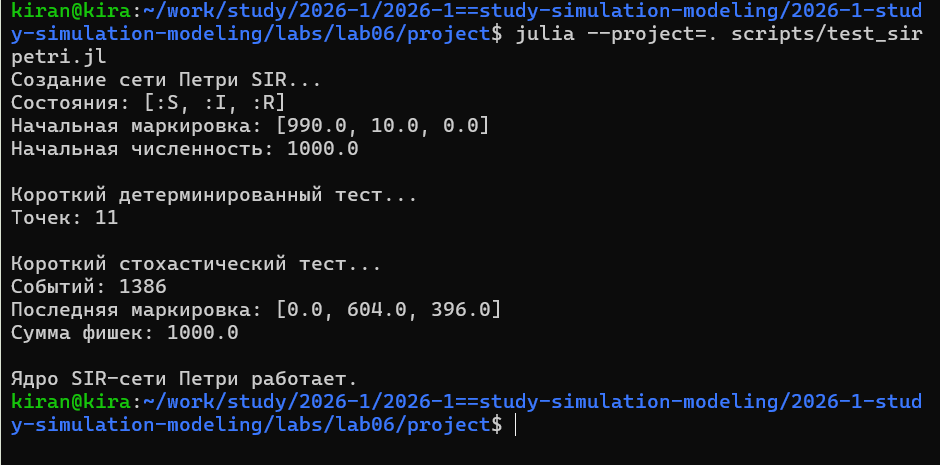
\includegraphics[width=0.95\linewidth,height=\textheight,keepaspectratio]{image/3.png}

}

\caption{Проверка ядра SIR-сети Петри}

\end{figure}%

В стохастической версии дополнительно контролируется сохранение общей
численности населения.

\chapter{Базовый
эксперимент}\label{ux431ux430ux437ux43eux432ux44bux439-ux44dux43aux441ux43fux435ux440ux438ux43cux435ux43dux442}

Для базового эксперимента использовались параметры:

\begin{itemize}
\tightlist
\item
  \texttt{β\ =\ 0.3};
\item
  \texttt{γ\ =\ 0.1};
\item
  \texttt{tmax\ =\ 100};
\item
  \texttt{seed\ =\ 123}.
\end{itemize}

Для одной и той же сети выполняются два вида моделирования.

Детерминированный вариант решает систему обыкновенных дифференциальных
уравнений и даёт непрерывную усреднённую динамику.

Стохастический вариант использует прямой алгоритм Гиллеспи, в котором
каждое заражение или выздоровление является отдельным случайным
событием.

\begin{figure}[H]

{\centering 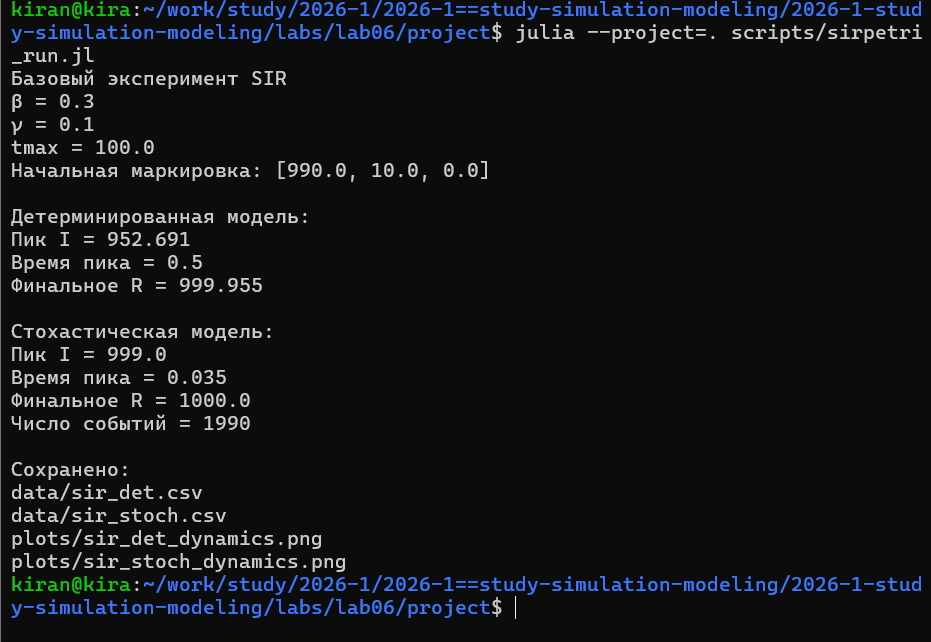
\includegraphics[width=0.95\linewidth,height=\textheight,keepaspectratio]{image/4.png}

}

\caption{Результаты базового эксперимента}

\end{figure}%

Для обеих траекторий программа автоматически определяет величину пика
инфицированных и время достижения максимума.

\begin{figure}[H]

{\centering 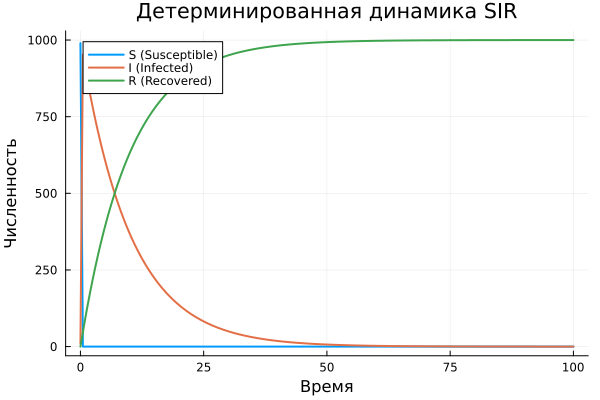
\includegraphics[width=0.9\linewidth,height=\textheight,keepaspectratio]{image/plots/sir_det_dynamics.png}

}

\caption{Детерминированная динамика SIR}

\end{figure}%

\begin{figure}[H]

{\centering 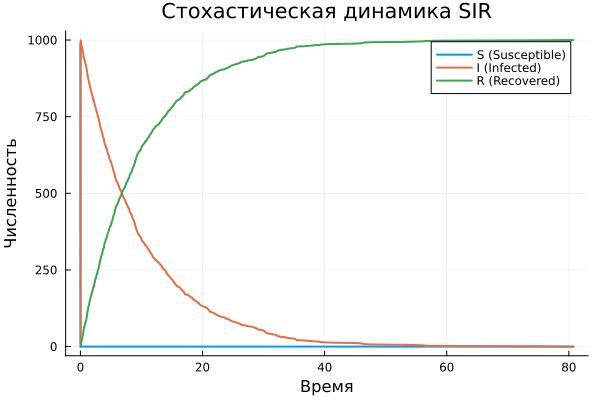
\includegraphics[width=0.9\linewidth,height=\textheight,keepaspectratio]{image/plots/sir_stoch_dynamics.png}

}

\caption{Стохастическая динамика SIR}

\end{figure}%

\chapter{Исследование коэффициента
заражения}\label{ux438ux441ux441ux43bux435ux434ux43eux432ux430ux43dux438ux435-ux43aux43eux44dux444ux444ux438ux446ux438ux435ux43dux442ux430-ux437ux430ux440ux430ux436ux435ux43dux438ux44f}

Для анализа чувствительности модели коэффициент выздоровления
фиксировался:

\texttt{γ\ =\ 0.1}.

Коэффициент заражения изменялся в диапазоне:

\texttt{β\ =\ 0.1\ :\ 0.05\ :\ 0.8}.

Для каждого значения выполнялась самостоятельная детерминированная
симуляция.

Программно рассчитывались:

\begin{itemize}
\tightlist
\item
  максимальное число инфицированных;
\item
  время пика;
\item
  итоговое число выздоровевших.
\end{itemize}

\begin{figure}[H]

{\centering 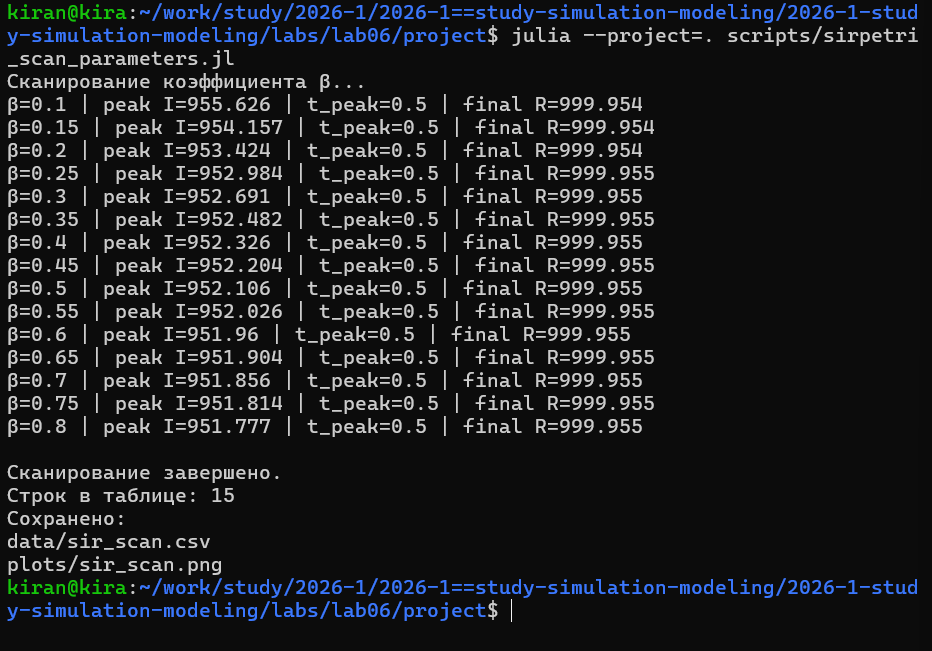
\includegraphics[width=0.95\linewidth,height=\textheight,keepaspectratio]{image/5.png}

}

\caption{Выполнение серии расчётов для различных β}

\end{figure}%

Всего было рассчитано 15 вариантов модели.

\begin{figure}[H]

{\centering 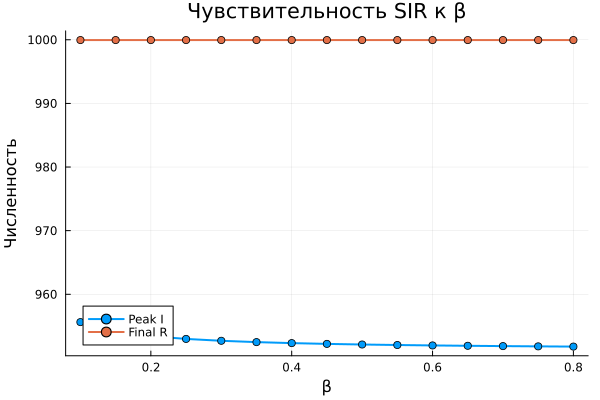
\includegraphics[width=0.9\linewidth,height=\textheight,keepaspectratio]{image/plots/sir_scan.png}

}

\caption{Чувствительность модели к коэффициенту β}

\end{figure}%

\chapter{Анимация
динамики}\label{ux430ux43dux438ux43cux430ux446ux438ux44f-ux434ux438ux43dux430ux43cux438ux43aux438}

Для динамической визуализации была создана GIF-анимация изменения
состояний \texttt{S}, \texttt{I} и \texttt{R}.

Сначала детерминированная траектория рассчитывалась с небольшим шагом
сохранения. Затем для анимации использовалась часть рассчитанных точек,
что позволяет уменьшить размер GIF без повторного вычисления модели.

\begin{figure}[H]

{\centering 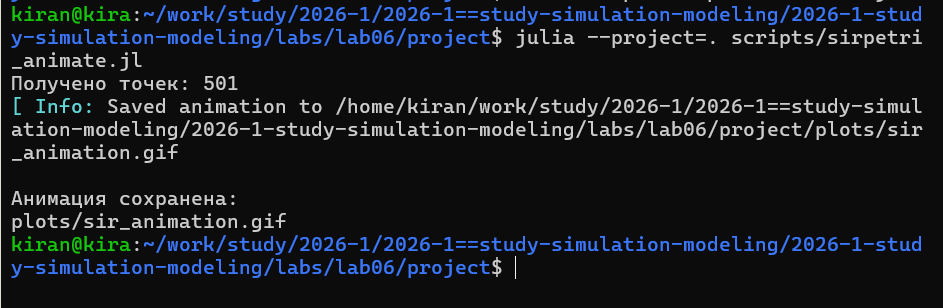
\includegraphics[width=0.95\linewidth,height=\textheight,keepaspectratio]{image/6.png}

}

\caption{Создание GIF-анимации}

\end{figure}%

Файл сохранён как:

\texttt{image/plots/sir\_animation.gif}.

\chapter{Итоговый сравнительный
анализ}\label{ux438ux442ux43eux433ux43eux432ux44bux439-ux441ux440ux430ux432ux43dux438ux442ux435ux43bux44cux43dux44bux439-ux430ux43dux430ux43bux438ux437}

Итоговый анализ выполнялся на основе уже сохранённых CSV-файлов.

Повторный запуск модели здесь не требуется.

Используются:

\begin{itemize}
\tightlist
\item
  \texttt{sir\_det.csv};
\item
  \texttt{sir\_stoch.csv};
\item
  \texttt{sir\_scan.csv}.
\end{itemize}

Сначала сравнивается динамика инфицированных в детерминированной и
стохастической моделях.

Затем отдельно строится зависимость максимального числа инфицированных
от коэффициента заражения.

\begin{figure}[H]

{\centering 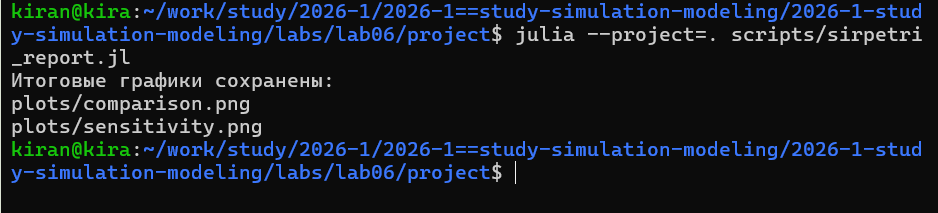
\includegraphics[width=0.95\linewidth,height=\textheight,keepaspectratio]{image/7.png}

}

\caption{Формирование итоговых графиков}

\end{figure}%

\begin{figure}[H]

{\centering 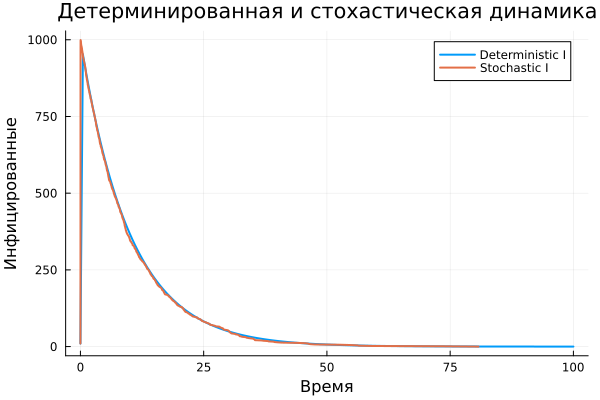
\includegraphics[width=0.9\linewidth,height=\textheight,keepaspectratio]{image/plots/comparison.png}

}

\caption{Сравнение детерминированной и стохастической динамики}

\end{figure}%

\begin{figure}[H]

{\centering 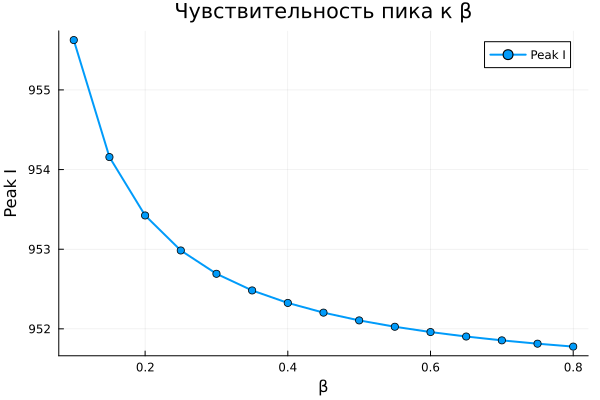
\includegraphics[width=0.9\linewidth,height=\textheight,keepaspectratio]{image/plots/sensitivity.png}

}

\caption{Чувствительность пика инфицированных к β}

\end{figure}%

\chapter{Параметрическое
исследование}\label{ux43fux430ux440ux430ux43cux435ux442ux440ux438ux447ux435ux441ux43aux43eux435-ux438ux441ux441ux43bux435ux434ux43eux432ux430ux43dux438ux435}

В дополнительной версии программы исследуется совместное влияние двух
параметров модели:

\begin{itemize}
\tightlist
\item
  коэффициента заражения \texttt{β};
\item
  коэффициента выздоровления \texttt{γ}.
\end{itemize}

Использовались значения:

\texttt{β\ =\ 0.1,\ 0.3,\ 0.5,\ 0.8};

\texttt{γ\ =\ 0.05,\ 0.10,\ 0.20}.

Всего получается 12 комбинаций.

Для каждой комбинации программа самостоятельно выполняет моделирование и
рассчитывает:

\begin{itemize}
\tightlist
\item
  пик инфицированных;
\item
  время пика;
\item
  итоговое число выздоровевших.
\end{itemize}

\begin{figure}[H]

{\centering 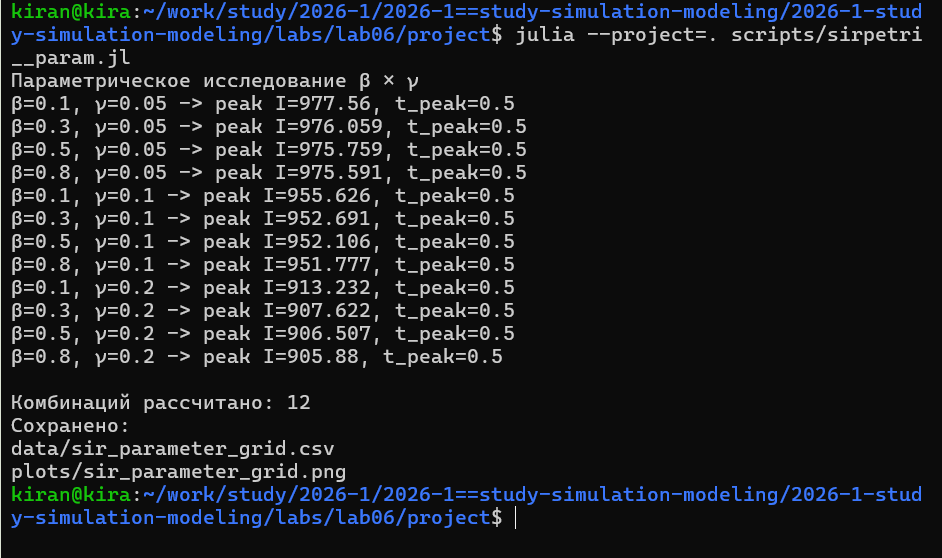
\includegraphics[width=0.95\linewidth,height=\textheight,keepaspectratio]{image/8.png}

}

\caption{Параметрическое исследование β и γ}

\end{figure}%

\begin{figure}[H]

{\centering 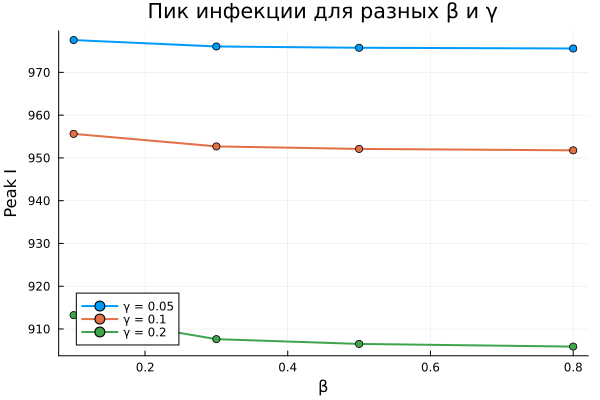
\includegraphics[width=0.9\linewidth,height=\textheight,keepaspectratio]{image/plots/sir_parameter_grid.png}

}

\caption{Пик инфицированных для различных β и γ}

\end{figure}%

Такой эксперимент позволяет исследовать совместное влияние скорости
заражения и скорости выздоровления, а не только изменение одного
параметра.

\chapter{Литературное
программирование}\label{ux43bux438ux442ux435ux440ux430ux442ux443ux440ux43dux43eux435-ux43fux440ux43eux433ux440ux430ux43cux43cux438ux440ux43eux432ux430ux43dux438ux435}

Основные вычислительные сценарии были оформлены в литературном стиле.

Из каждого исходника автоматически создавались:

\begin{itemize}
\tightlist
\item
  чистый Julia-код;
\item
  Jupyter Notebook;
\item
  документация Quarto.
\end{itemize}

\begin{figure}[H]

{\centering 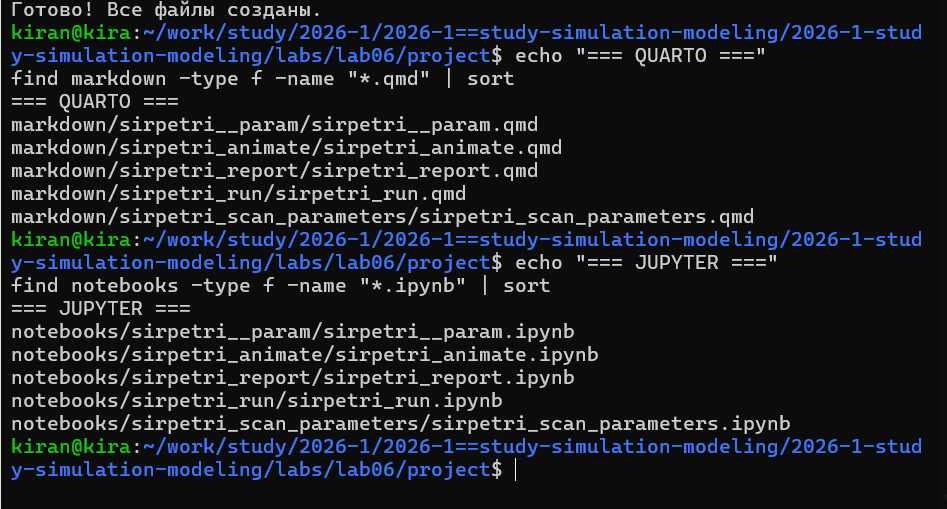
\includegraphics[width=0.95\linewidth,height=\textheight,keepaspectratio]{image/9.png}

}

\caption{Сгенерированные Quarto-документы и Jupyter Notebook}

\end{figure}%

\chapter{Проверка
воспроизводимости}\label{ux43fux440ux43eux432ux435ux440ux43aux430-ux432ux43eux441ux43fux440ux43eux438ux437ux432ux43eux434ux438ux43cux43eux441ux442ux438}

После генерации все Jupyter Notebook были отдельно выполнены.

Таким образом проверяется, что автоматически созданные notebooks
содержат все необходимые действия и способны самостоятельно повторить
вычислительные эксперименты.

\begin{figure}[H]

{\centering 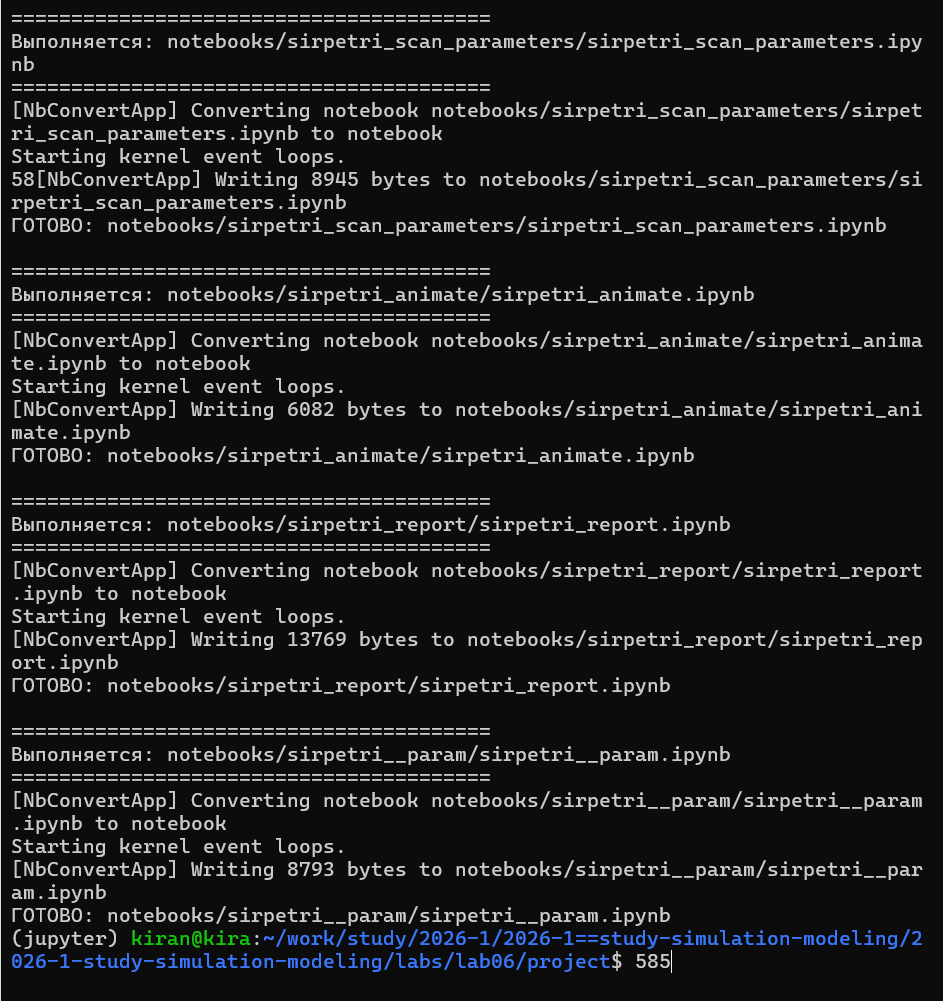
\includegraphics[width=0.95\linewidth,height=\textheight,keepaspectratio]{image/10.png}

}

\caption{Успешное выполнение Jupyter Notebook}

\end{figure}%

\chapter{Структура
проекта}\label{ux441ux442ux440ux443ux43aux442ux443ux440ux430-ux43fux440ux43eux435ux43aux442ux430}

После выполнения лабораторной работы проект содержит:

\begin{itemize}
\tightlist
\item
  модуль \texttt{SIRPetri};
\item
  литературные программы;
\item
  сгенерированный Julia-код;
\item
  Jupyter Notebook;
\item
  Quarto-документацию;
\item
  CSV-файлы;
\item
  оригинальные PNG-графики;
\item
  GIF-анимацию.
\end{itemize}

\begin{figure}[H]

{\centering 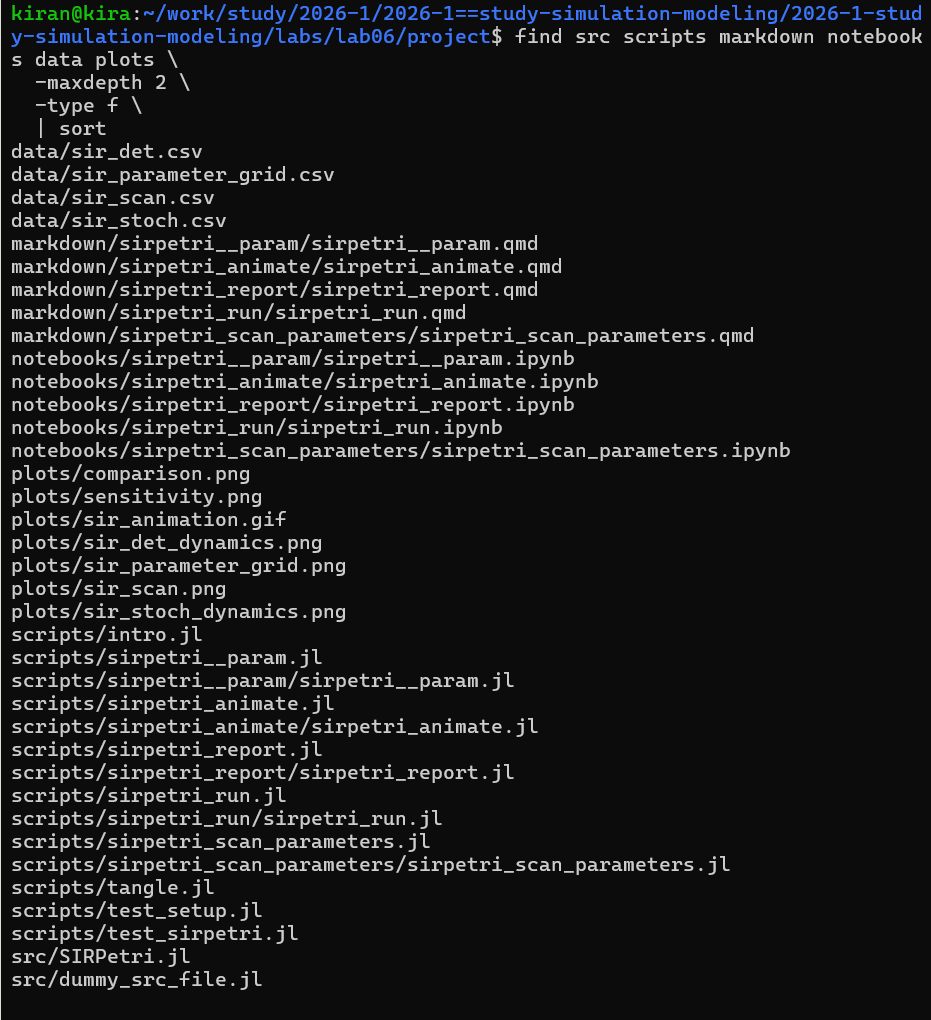
\includegraphics[width=0.95\linewidth,height=\textheight,keepaspectratio]{image/11.png}

}

\caption{Итоговая структура проекта}

\end{figure}%

\chapter{Контроль
версий}\label{ux43aux43eux43dux442ux440ux43eux43bux44c-ux432ux435ux440ux441ux438ux439}

Все материалы лабораторной работы были сохранены в Git и отправлены в
удалённые репозитории GitVerse и GitHub.

\begin{figure}[H]

{\centering 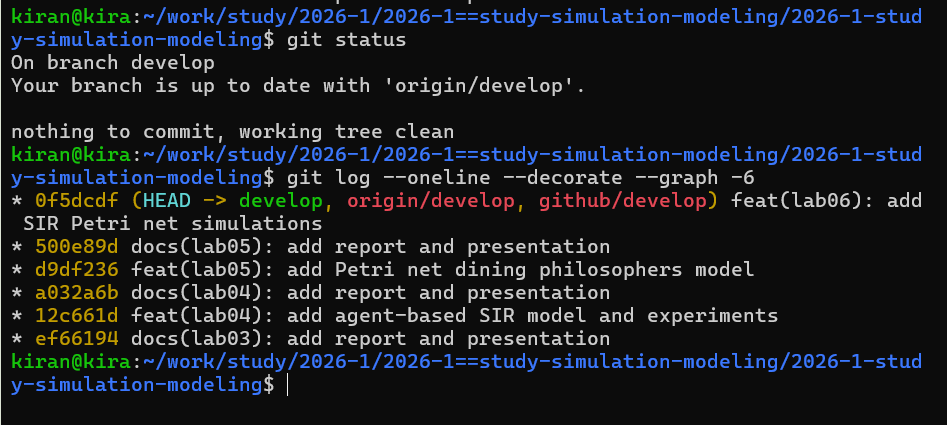
\includegraphics[width=0.95\linewidth,height=\textheight,keepaspectratio]{image/12.png}

}

\caption{Финальное состояние Git}

\end{figure}%

\chapter{Выводы}\label{ux432ux44bux432ux43eux434ux44b}

В лабораторной работе модель SIR была представлена в форме сети Петри.

Переход заражения изменяет маркировку между состояниями \texttt{S} и
\texttt{I}, а переход выздоровления переводит фишки из \texttt{I} в
\texttt{R}.

Для одной модели были реализованы два способа моделирования.
Детерминированный подход использует систему ОДУ и описывает усреднённую
непрерывную динамику. Стохастический подход моделирует отдельные
случайные события с помощью алгоритма Гиллеспи.

Дополнительно было исследовано влияние коэффициента заражения и
совместное влияние параметров \texttt{β} и \texttt{γ}.

Результаты вычислений сохраняются отдельно от анализа, что позволяет
повторно использовать CSV-файлы без повторного запуска модели.

Все основные вычислительные сценарии оформлены в литературном стиле, а
автоматически созданные notebooks выполнены для проверки
воспроизводимости.

\chapter*{Приложение А. Quarto-документация базового
эксперимента}\label{ux43fux440ux438ux43bux43eux436ux435ux43dux438ux435-ux430.-quarto-ux434ux43eux43aux443ux43cux435ux43dux442ux430ux446ux438ux44f-ux431ux430ux437ux43eux432ux43eux433ux43e-ux44dux43aux441ux43fux435ux440ux438ux43cux435ux43dux442ux430}
\addcontentsline{toc}{chapter}{Приложение А. Quarto-документация
базового эксперимента}

Ниже интегрирована статическая версия Quarto-документации, автоматически
полученной из литературного исходного кода.

\chapter{Базовый эксперимент SIR в сети
Петри}\label{ux431ux430ux437ux43eux432ux44bux439-ux44dux43aux441ux43fux435ux440ux438ux43cux435ux43dux442-sir-ux432-ux441ux435ux442ux438-ux43fux435ux442ux440ux438}

\textbf{Автор:} Нечаева Кира Андреевна

\textbf{Группа:} НКНбд-01-23

Выполняется сравнение детерминированной и стохастической динамики одной
модели.

\begin{Shaded}
\begin{Highlighting}[]
\ConstantTok{ENV}\NormalTok{[}\StringTok{"GKSwstype"}\NormalTok{] }\OperatorTok{=} \StringTok{"100"}

\ImportTok{using} \BuiltInTok{DrWatson}
\PreprocessorTok{@quickactivate} \StringTok{"project"}

\ImportTok{using} \BuiltInTok{Random}
\ImportTok{using} \BuiltInTok{DataFrames}
\ImportTok{using} \BuiltInTok{CSV}
\ImportTok{using} \BuiltInTok{Plots}

\FunctionTok{include}\NormalTok{(}
    \FunctionTok{srcdir}\NormalTok{(}
        \StringTok{"SIRPetri.jl"}
\NormalTok{    )}
\NormalTok{)}

\ImportTok{using} \BuiltInTok{.SIRPetri}
\end{Highlighting}
\end{Shaded}

\section{Параметры}\label{ux43fux430ux440ux430ux43cux435ux442ux440ux44b}

\begin{Shaded}
\begin{Highlighting}[]
\NormalTok{β }\OperatorTok{=}
    \FloatTok{0.3}

\NormalTok{γ }\OperatorTok{=}
    \FloatTok{0.1}

\NormalTok{tmax }\OperatorTok{=}
    \FloatTok{100.0}

\NormalTok{seed }\OperatorTok{=}
    \FloatTok{123}

\FunctionTok{println}\NormalTok{(}
    \StringTok{"Базовый эксперимент SIR"}
\NormalTok{)}

\FunctionTok{println}\NormalTok{(}
    \StringTok{"β = "}\NormalTok{,}
\NormalTok{    β}
\NormalTok{)}

\FunctionTok{println}\NormalTok{(}
    \StringTok{"γ = "}\NormalTok{,}
\NormalTok{    γ}
\NormalTok{)}

\FunctionTok{println}\NormalTok{(}
    \StringTok{"tmax = "}\NormalTok{,}
\NormalTok{    tmax}
\NormalTok{)}
\end{Highlighting}
\end{Shaded}

\section{Построение
сети}\label{ux43fux43eux441ux442ux440ux43eux435ux43dux438ux435-ux441ux435ux442ux438}

\begin{Shaded}
\begin{Highlighting}[]
\NormalTok{net,}
\NormalTok{u0,}
\NormalTok{states }\OperatorTok{=}
    \FunctionTok{build\_sir\_network}\NormalTok{(}
\NormalTok{        β,}
\NormalTok{        γ}
\NormalTok{    )}

\FunctionTok{println}\NormalTok{(}
    \StringTok{"Начальная маркировка: "}\NormalTok{,}
\NormalTok{    u0}
\NormalTok{)}
\end{Highlighting}
\end{Shaded}

\section{Детерминированная
симуляция}\label{ux434ux435ux442ux435ux440ux43cux438ux43dux438ux440ux43eux432ux430ux43dux43dux430ux44f-ux441ux438ux43cux443ux43bux44fux446ux438ux44f}

\begin{Shaded}
\begin{Highlighting}[]
\NormalTok{df\_det }\OperatorTok{=}
    \FunctionTok{simulate\_deterministic}\NormalTok{(}
\NormalTok{        net,}
\NormalTok{        u0,}
\NormalTok{        (}
            \FloatTok{0.0}\NormalTok{,}
\NormalTok{            tmax}
\NormalTok{        );}
\NormalTok{        saveat}\OperatorTok{=}\FloatTok{0.5}\NormalTok{,}
\NormalTok{        rates}\OperatorTok{=}\NormalTok{[}
\NormalTok{            β,}
\NormalTok{            γ}
\NormalTok{        ]}
\NormalTok{    )}

\NormalTok{CSV.}\FunctionTok{write}\NormalTok{(}
    \FunctionTok{datadir}\NormalTok{(}
        \StringTok{"sir\_det.csv"}
\NormalTok{    ),}
\NormalTok{    df\_det}
\NormalTok{)}

\NormalTok{peak\_det\_index }\OperatorTok{=}
    \FunctionTok{argmax}\NormalTok{(}
\NormalTok{        df\_det.I}
\NormalTok{    )}

\NormalTok{peak\_det }\OperatorTok{=}
\NormalTok{    df\_det.I[}
\NormalTok{        peak\_det\_index}
\NormalTok{    ]}

\NormalTok{peak\_det\_time }\OperatorTok{=}
\NormalTok{    df\_det.time[}
\NormalTok{        peak\_det\_index}
\NormalTok{    ]}

\FunctionTok{println}\NormalTok{(}
    \StringTok{"}\SpecialCharTok{\textbackslash{}n}\StringTok{Детерминированная модель:"}
\NormalTok{)}

\FunctionTok{println}\NormalTok{(}
    \StringTok{"Пик I = "}\NormalTok{,}
    \FunctionTok{round}\NormalTok{(}
\NormalTok{        peak\_det,}
\NormalTok{        digits}\OperatorTok{=}\FloatTok{3}
\NormalTok{    )}
\NormalTok{)}

\FunctionTok{println}\NormalTok{(}
    \StringTok{"Время пика = "}\NormalTok{,}
    \FunctionTok{round}\NormalTok{(}
\NormalTok{        peak\_det\_time,}
\NormalTok{        digits}\OperatorTok{=}\FloatTok{3}
\NormalTok{    )}
\NormalTok{)}

\FunctionTok{println}\NormalTok{(}
    \StringTok{"Финальное R = "}\NormalTok{,}
    \FunctionTok{round}\NormalTok{(}
\NormalTok{        df\_det.R[}\KeywordTok{end}\NormalTok{],}
\NormalTok{        digits}\OperatorTok{=}\FloatTok{3}
\NormalTok{    )}
\NormalTok{)}

\NormalTok{p\_det }\OperatorTok{=}
    \FunctionTok{plot\_sir}\NormalTok{(}
\NormalTok{        df\_det;}
\NormalTok{        title}\OperatorTok{=}
            \StringTok{"Детерминированная динамика SIR"}
\NormalTok{    )}

\FunctionTok{savefig}\NormalTok{(}
\NormalTok{    p\_det,}
    \FunctionTok{plotsdir}\NormalTok{(}
        \StringTok{"sir\_det\_dynamics.png"}
\NormalTok{    )}
\NormalTok{)}
\end{Highlighting}
\end{Shaded}

\section{Стохастическая
симуляция}\label{ux441ux442ux43eux445ux430ux441ux442ux438ux447ux435ux441ux43aux430ux44f-ux441ux438ux43cux443ux43bux44fux446ux438ux44f}

\begin{Shaded}
\begin{Highlighting}[]
\NormalTok{rng }\OperatorTok{=}
    \FunctionTok{MersenneTwister}\NormalTok{(}
\NormalTok{        seed}
\NormalTok{    )}

\NormalTok{df\_stoch }\OperatorTok{=}
    \FunctionTok{simulate\_stochastic}\NormalTok{(}
\NormalTok{        net,}
\NormalTok{        u0,}
\NormalTok{        (}
            \FloatTok{0.0}\NormalTok{,}
\NormalTok{            tmax}
\NormalTok{        );}
\NormalTok{        rates}\OperatorTok{=}\NormalTok{[}
\NormalTok{            β,}
\NormalTok{            γ}
\NormalTok{        ],}
\NormalTok{        rng}\OperatorTok{=}\NormalTok{rng}
\NormalTok{    )}

\NormalTok{CSV.}\FunctionTok{write}\NormalTok{(}
    \FunctionTok{datadir}\NormalTok{(}
        \StringTok{"sir\_stoch.csv"}
\NormalTok{    ),}
\NormalTok{    df\_stoch}
\NormalTok{)}

\NormalTok{peak\_stoch\_index }\OperatorTok{=}
    \FunctionTok{argmax}\NormalTok{(}
\NormalTok{        df\_stoch.I}
\NormalTok{    )}

\NormalTok{peak\_stoch }\OperatorTok{=}
\NormalTok{    df\_stoch.I[}
\NormalTok{        peak\_stoch\_index}
\NormalTok{    ]}

\NormalTok{peak\_stoch\_time }\OperatorTok{=}
\NormalTok{    df\_stoch.time[}
\NormalTok{        peak\_stoch\_index}
\NormalTok{    ]}

\FunctionTok{println}\NormalTok{(}
    \StringTok{"}\SpecialCharTok{\textbackslash{}n}\StringTok{Стохастическая модель:"}
\NormalTok{)}

\FunctionTok{println}\NormalTok{(}
    \StringTok{"Пик I = "}\NormalTok{,}
\NormalTok{    peak\_stoch}
\NormalTok{)}

\FunctionTok{println}\NormalTok{(}
    \StringTok{"Время пика = "}\NormalTok{,}
    \FunctionTok{round}\NormalTok{(}
\NormalTok{        peak\_stoch\_time,}
\NormalTok{        digits}\OperatorTok{=}\FloatTok{3}
\NormalTok{    )}
\NormalTok{)}

\FunctionTok{println}\NormalTok{(}
    \StringTok{"Финальное R = "}\NormalTok{,}
\NormalTok{    df\_stoch.R[}\KeywordTok{end}\NormalTok{]}
\NormalTok{)}

\FunctionTok{println}\NormalTok{(}
    \StringTok{"Число событий = "}\NormalTok{,}
    \FunctionTok{nrow}\NormalTok{(df\_stoch) }\OperatorTok{{-}} \FloatTok{1}
\NormalTok{)}

\NormalTok{p\_stoch }\OperatorTok{=}
    \FunctionTok{plot\_sir}\NormalTok{(}
\NormalTok{        df\_stoch;}
\NormalTok{        title}\OperatorTok{=}
            \StringTok{"Стохастическая динамика SIR"}
\NormalTok{    )}

\FunctionTok{savefig}\NormalTok{(}
\NormalTok{    p\_stoch,}
    \FunctionTok{plotsdir}\NormalTok{(}
        \StringTok{"sir\_stoch\_dynamics.png"}
\NormalTok{    )}
\NormalTok{)}
\end{Highlighting}
\end{Shaded}

\section{Результаты}\label{ux440ux435ux437ux443ux43bux44cux442ux430ux442ux44b}

\begin{Shaded}
\begin{Highlighting}[]
\FunctionTok{println}\NormalTok{(}
    \StringTok{"}\SpecialCharTok{\textbackslash{}n}\StringTok{Сохранено:"}
\NormalTok{)}

\FunctionTok{println}\NormalTok{(}
    \StringTok{"data/sir\_det.csv"}
\NormalTok{)}

\FunctionTok{println}\NormalTok{(}
    \StringTok{"data/sir\_stoch.csv"}
\NormalTok{)}

\FunctionTok{println}\NormalTok{(}
    \StringTok{"plots/sir\_det\_dynamics.png"}
\NormalTok{)}

\FunctionTok{println}\NormalTok{(}
    \StringTok{"plots/sir\_stoch\_dynamics.png"}
\NormalTok{)}
\end{Highlighting}
\end{Shaded}

\section{Вывод}\label{ux432ux44bux432ux43eux434}

Детерминированная модель показывает усреднённую непрерывную динамику, а
алгоритм Гиллеспи моделирует отдельные случайные события.

\chapter*{Приложение Б. Quarto-документация параметрического
эксперимента}\label{ux43fux440ux438ux43bux43eux436ux435ux43dux438ux435-ux431.-quarto-ux434ux43eux43aux443ux43cux435ux43dux442ux430ux446ux438ux44f-ux43fux430ux440ux430ux43cux435ux442ux440ux438ux447ux435ux441ux43aux43eux433ux43e-ux44dux43aux441ux43fux435ux440ux438ux43cux435ux43dux442ux430}
\addcontentsline{toc}{chapter}{Приложение Б. Quarto-документация
параметрического эксперимента}

Ниже интегрирована статическая версия документации параметрической
программы.

\chapter{Параметрическое исследование
SIR}\label{ux43fux430ux440ux430ux43cux435ux442ux440ux438ux447ux435ux441ux43aux43eux435-ux438ux441ux441ux43bux435ux434ux43eux432ux430ux43dux438ux435-sir}

\textbf{Автор:} Нечаева Кира Андреевна

\textbf{Группа:} НКНбд-01-23

Исследуются комбинации двух параметров: коэффициента заражения β и
коэффициента выздоровления γ.

\begin{Shaded}
\begin{Highlighting}[]
\ConstantTok{ENV}\NormalTok{[}\StringTok{"GKSwstype"}\NormalTok{] }\OperatorTok{=} \StringTok{"100"}

\ImportTok{using} \BuiltInTok{DrWatson}
\PreprocessorTok{@quickactivate} \StringTok{"project"}

\ImportTok{using} \BuiltInTok{DataFrames}
\ImportTok{using} \BuiltInTok{CSV}
\ImportTok{using} \BuiltInTok{Plots}

\FunctionTok{include}\NormalTok{(}
    \FunctionTok{srcdir}\NormalTok{(}
        \StringTok{"SIRPetri.jl"}
\NormalTok{    )}
\NormalTok{)}

\ImportTok{using} \BuiltInTok{.SIRPetri}
\end{Highlighting}
\end{Shaded}

\section{Наборы
параметров}\label{ux43dux430ux431ux43eux440ux44b-ux43fux430ux440ux430ux43cux435ux442ux440ux43eux432}

\begin{Shaded}
\begin{Highlighting}[]
\NormalTok{β\_values }\OperatorTok{=}
\NormalTok{    [}
        \FloatTok{0.1}\NormalTok{,}
        \FloatTok{0.3}\NormalTok{,}
        \FloatTok{0.5}\NormalTok{,}
        \FloatTok{0.8}
\NormalTok{    ]}

\NormalTok{γ\_values }\OperatorTok{=}
\NormalTok{    [}
        \FloatTok{0.05}\NormalTok{,}
        \FloatTok{0.10}\NormalTok{,}
        \FloatTok{0.20}
\NormalTok{    ]}

\NormalTok{tmax }\OperatorTok{=}
    \FloatTok{100.0}

\NormalTok{results }\OperatorTok{=}
    \DataTypeTok{NamedTuple}\NormalTok{[]}

\FunctionTok{println}\NormalTok{(}
    \StringTok{"Параметрическое исследование β × γ"}
\NormalTok{)}
\end{Highlighting}
\end{Shaded}

\section{Серия
расчётов}\label{ux441ux435ux440ux438ux44f-ux440ux430ux441ux447ux451ux442ux43eux432}

\begin{Shaded}
\begin{Highlighting}[]
\ControlFlowTok{for}\NormalTok{ γ }\KeywordTok{in}\NormalTok{ γ\_values}

    \ControlFlowTok{for}\NormalTok{ β }\KeywordTok{in}\NormalTok{ β\_values}

\NormalTok{        net,}
\NormalTok{        u0,}
\NormalTok{        \_ }\OperatorTok{=}
            \FunctionTok{build\_sir\_network}\NormalTok{(}
\NormalTok{                β,}
\NormalTok{                γ}
\NormalTok{            )}

\NormalTok{        df }\OperatorTok{=}
            \FunctionTok{simulate\_deterministic}\NormalTok{(}
\NormalTok{                net,}
\NormalTok{                u0,}
\NormalTok{                (}
                    \FloatTok{0.0}\NormalTok{,}
\NormalTok{                    tmax}
\NormalTok{                );}
\NormalTok{                saveat}\OperatorTok{=}\FloatTok{0.5}\NormalTok{,}
\NormalTok{                rates}\OperatorTok{=}\NormalTok{[}
\NormalTok{                    β,}
\NormalTok{                    γ}
\NormalTok{                ]}
\NormalTok{            )}

\NormalTok{        peak\_index }\OperatorTok{=}
            \FunctionTok{argmax}\NormalTok{(}
\NormalTok{                df.I}
\NormalTok{            )}

\NormalTok{        peak\_I }\OperatorTok{=}
\NormalTok{            df.I[}
\NormalTok{                peak\_index}
\NormalTok{            ]}

\NormalTok{        peak\_time }\OperatorTok{=}
\NormalTok{            df.time[}
\NormalTok{                peak\_index}
\NormalTok{            ]}

\NormalTok{        final\_R }\OperatorTok{=}
\NormalTok{            df.R[}\KeywordTok{end}\NormalTok{]}

        \FunctionTok{push!}\NormalTok{(}
\NormalTok{            results,}
\NormalTok{            (}
\NormalTok{                β}\OperatorTok{=}\NormalTok{β,}
\NormalTok{                γ}\OperatorTok{=}\NormalTok{γ,}
\NormalTok{                peak\_I}\OperatorTok{=}\NormalTok{peak\_I,}
\NormalTok{                peak\_time}\OperatorTok{=}\NormalTok{peak\_time,}
\NormalTok{                final\_R}\OperatorTok{=}\NormalTok{final\_R}
\NormalTok{            )}
\NormalTok{        )}

        \FunctionTok{println}\NormalTok{(}
            \StringTok{"β="}\NormalTok{,}
\NormalTok{            β,}
            \StringTok{", γ="}\NormalTok{,}
\NormalTok{            γ,}
            \StringTok{" {-}\textgreater{} peak I="}\NormalTok{,}
            \FunctionTok{round}\NormalTok{(}
\NormalTok{                peak\_I,}
\NormalTok{                digits}\OperatorTok{=}\FloatTok{3}
\NormalTok{            ),}
            \StringTok{", t\_peak="}\NormalTok{,}
            \FunctionTok{round}\NormalTok{(}
\NormalTok{                peak\_time,}
\NormalTok{                digits}\OperatorTok{=}\FloatTok{3}
\NormalTok{            )}
\NormalTok{        )}
    \ControlFlowTok{end}
\ControlFlowTok{end}
\end{Highlighting}
\end{Shaded}

\section{Таблица}\label{ux442ux430ux431ux43bux438ux446ux430}

\begin{Shaded}
\begin{Highlighting}[]
\NormalTok{df\_params }\OperatorTok{=}
    \FunctionTok{DataFrame}\NormalTok{(}
\NormalTok{        results}
\NormalTok{    )}

\NormalTok{CSV.}\FunctionTok{write}\NormalTok{(}
    \FunctionTok{datadir}\NormalTok{(}
        \StringTok{"sir\_parameter\_grid.csv"}
\NormalTok{    ),}
\NormalTok{    df\_params}
\NormalTok{)}

\FunctionTok{println}\NormalTok{(}
    \StringTok{"}\SpecialCharTok{\textbackslash{}n}\StringTok{Комбинаций рассчитано: "}\NormalTok{,}
    \FunctionTok{nrow}\NormalTok{(df\_params)}
\NormalTok{)}
\end{Highlighting}
\end{Shaded}

\section{График}\label{ux433ux440ux430ux444ux438ux43a}

\begin{Shaded}
\begin{Highlighting}[]
\NormalTok{p }\OperatorTok{=}
    \FunctionTok{plot}\NormalTok{(}
\NormalTok{        xlabel}\OperatorTok{=}\StringTok{"β"}\NormalTok{,}
\NormalTok{        ylabel}\OperatorTok{=}\StringTok{"Peak I"}\NormalTok{,}
\NormalTok{        title}\OperatorTok{=}
            \StringTok{"Пик инфекции для разных β и γ"}
\NormalTok{    )}

\ControlFlowTok{for}\NormalTok{ γ }\KeywordTok{in}\NormalTok{ γ\_values}

\NormalTok{    part }\OperatorTok{=}
        \FunctionTok{filter}\NormalTok{(}
            \OperatorTok{:}\NormalTok{γ }\OperatorTok{=\textgreater{}}
\NormalTok{                value }\OperatorTok{{-}\textgreater{}}
\NormalTok{                    value }\OperatorTok{==}\NormalTok{ γ,}
\NormalTok{            df\_params}
\NormalTok{        )}

    \FunctionTok{plot!}\NormalTok{(}
\NormalTok{        p,}
\NormalTok{        part.β,}
\NormalTok{        part.peak\_I;}
\NormalTok{        marker}\OperatorTok{=:}\NormalTok{circle,}
\NormalTok{        linewidth}\OperatorTok{=}\FloatTok{2}\NormalTok{,}
\NormalTok{        label}\OperatorTok{=}
            \StringTok{"γ = }\SpecialCharTok{$}\StringTok{γ"}
\StringTok{    )}
\NormalTok{end}

\FunctionTok{savefig}\NormalTok{(}
\NormalTok{    p,}
    \FunctionTok{plotsdir}\NormalTok{(}
        \StringTok{"sir\_parameter\_grid.png"}
\NormalTok{    )}
\NormalTok{)}

\FunctionTok{println}\NormalTok{(}
    \StringTok{"Сохранено:"}
\NormalTok{)}

\FunctionTok{println}\NormalTok{(}
    \StringTok{"data/sir\_parameter\_grid.csv"}
\NormalTok{)}

\FunctionTok{println}\NormalTok{(}
    \StringTok{"plots/sir\_parameter\_grid.png"}
\NormalTok{)}
\end{Highlighting}
\end{Shaded}

\section{Вывод}\label{ux432ux44bux432ux43eux434-1}

Использование сетки параметров позволяет сравнивать совместное влияние
скорости заражения и скорости выздоровления.


\printbibliography



\end{document}
